\section{Simulations}
%
% \begin{figure*}[ht]
%   \centering
%   \subfloat[Configuration $q$]{\includegraphics[width=0.33\textwidth]{figures/time_series_plot_m_p-0.5_untuned_configuration_v2.eps}\label{fig:time_series_plot_m_p_0.5_configuration}}
%   \subfloat[Piston position $\mu_\mathrm{p}$]{\includegraphics[width=0.33\textwidth]{figures/time_series_plot_m_p-0.5_untuned_piston_position_v2.eps}\label{fig:time_series_plot_m_p_0.5_piston_position}}
%   \subfloat[Actuation force $f_\mathrm{p}$]{\includegraphics[width=0.33\textwidth]{figures/time_series_plot_m_p-0.5_untuned_actuation_force_v2.eps}\label{fig:time_series_plot_m_p_0.5_actuation_force}}\\
%   \caption{Simulation of posture regulation under \gls{PCC} approximation for an actuation system with increased inertia ($m_\mathrm{p} = \SI{0.5}{kg}$) comparing the performance of the nonlinear backstepping controller (dashed lines) with a PID baseline controller (dotted lines). The set-point reference configuration is shown with solid lines. All gains remain unchanged and are tuned for the original system with $m_\mathrm{p} = \SI{0.19}{kg}$.}
% \end{figure*}
\begin{figure*}[ht]
  \centering
  \captionsetup[subfigure]{labelformat=empty}
  % End-to-end PID
  \subfloat{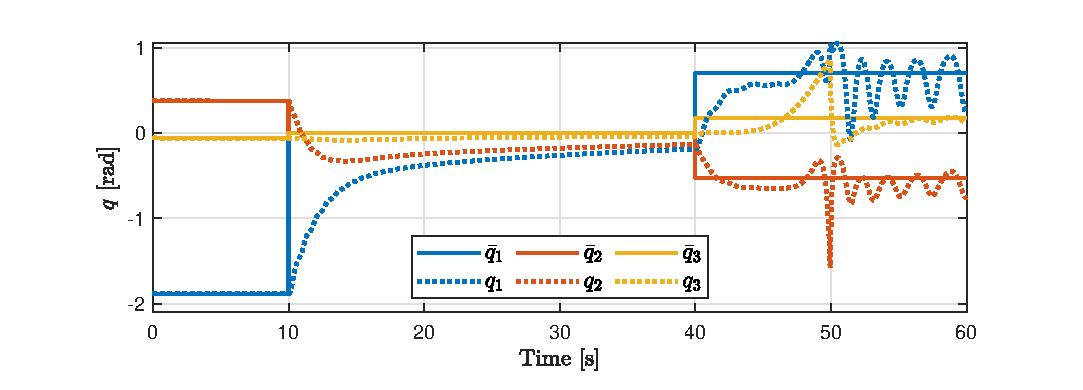
\includegraphics[width=0.33\textwidth, trim={0.75cm 0.85cm 0.75cm 0cm}]{backstepping/figures/time_series_plot_m_p-0.5_untuned_configuration_full_system_PID_v2.eps}}
  \subfloat{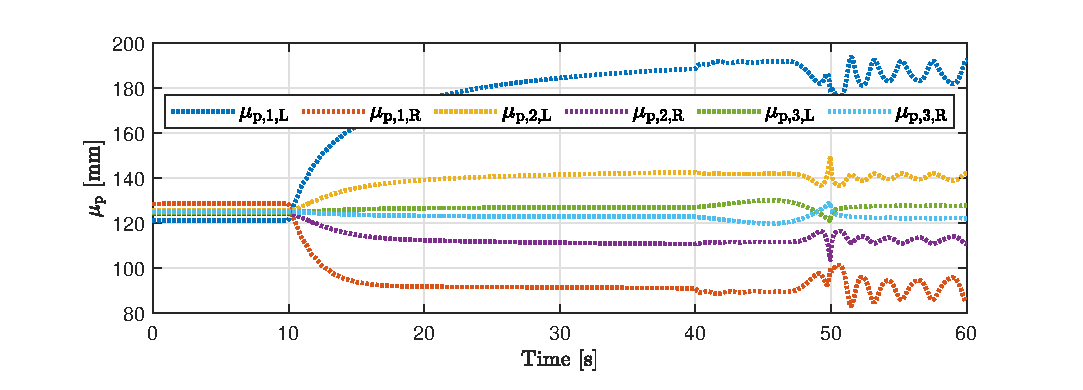
\includegraphics[width=0.33\textwidth, trim={0.75cm 0.85cm 0.75cm 0cm}]{backstepping/figures/time_series_plot_m_p-0.5_untuned_piston_position_full_system_PID_v2.eps}}
  \subfloat{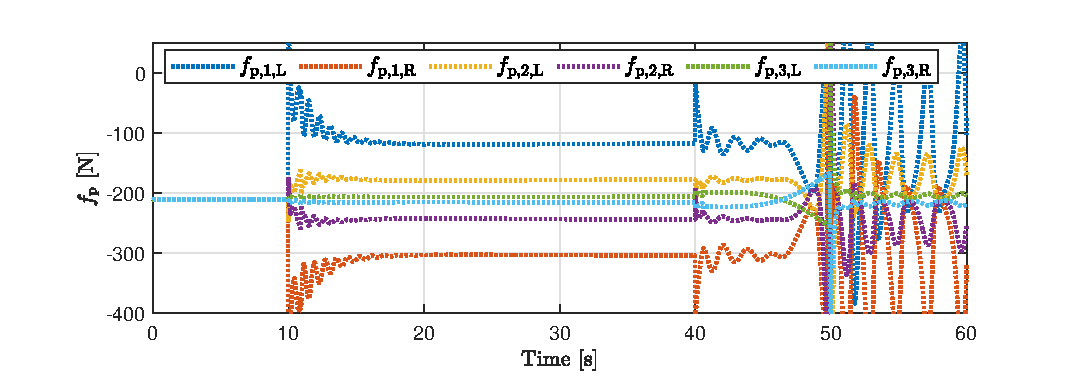
\includegraphics[width=0.33\textwidth, trim={0.75cm 0.85cm 0.75cm 0cm}]{backstepping/figures/time_series_plot_m_p-0.5_untuned_actuation_force_full_system_PID_v2.eps}}\\
  % Coupling-aware PID
  \subfloat{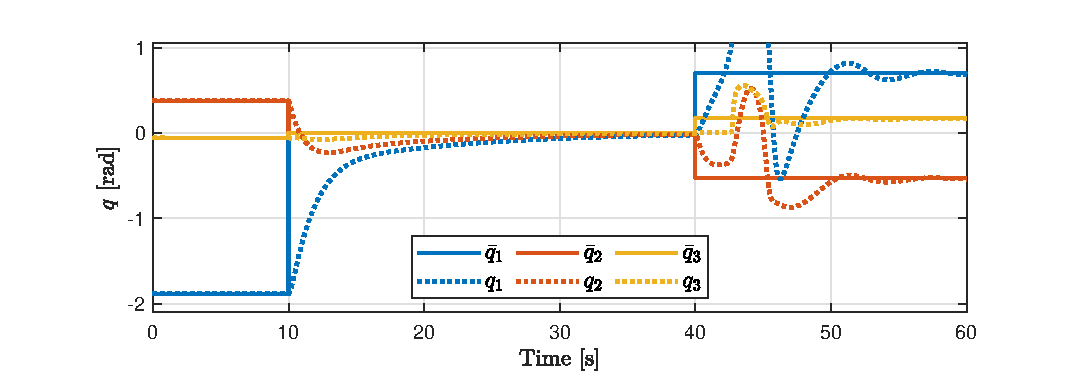
\includegraphics[width=0.33\textwidth, trim={0.75cm 0.87cm 0.75cm 0cm}]{backstepping/figures/time_series_plot_m_p-0.5_untuned_configuration_coupling_aware_PID_v2.eps}}
  \subfloat{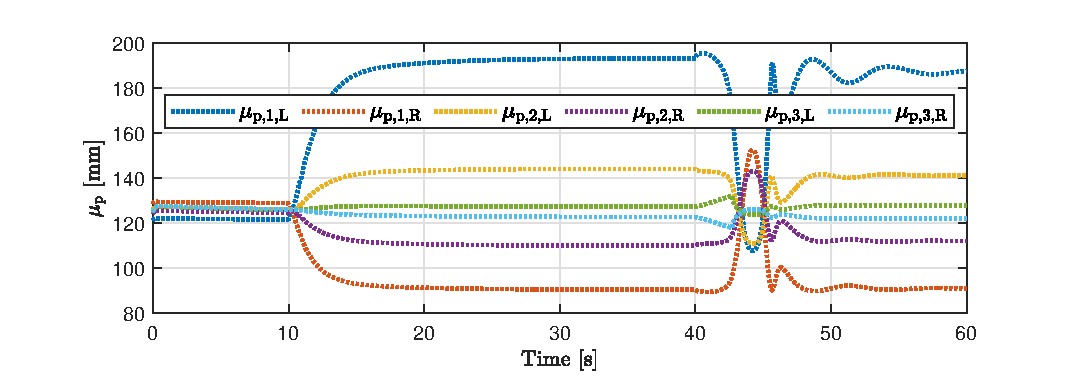
\includegraphics[width=0.33\textwidth, trim={0.75cm 0.87cm 0.75cm 0cm}]{backstepping/figures/time_series_plot_m_p-0.5_untuned_piston_position_coupling_aware_PID_v2.eps}}
  \subfloat{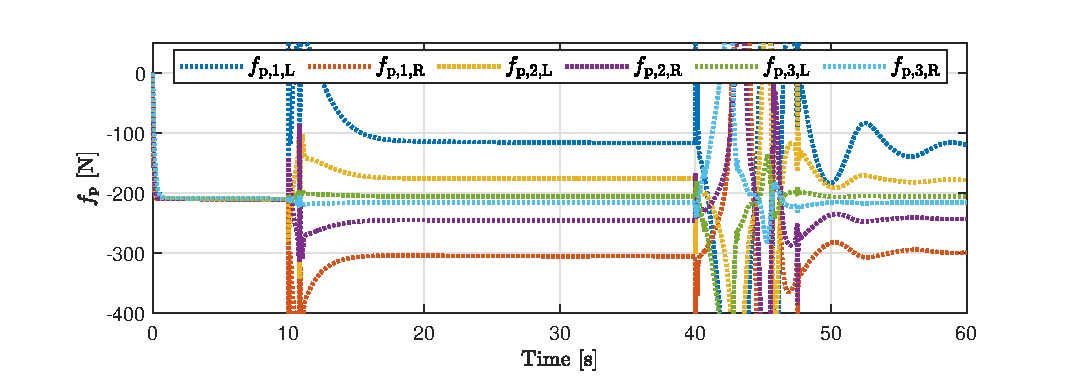
\includegraphics[width=0.33\textwidth, trim={0.75cm 0.87cm 0.75cm 0cm}]{backstepping/figures/time_series_plot_m_p-0.5_untuned_actuation_force_coupling_aware_PID_v2.eps}}\\
  % Backstepping
  \subfloat[Configuration $q$]{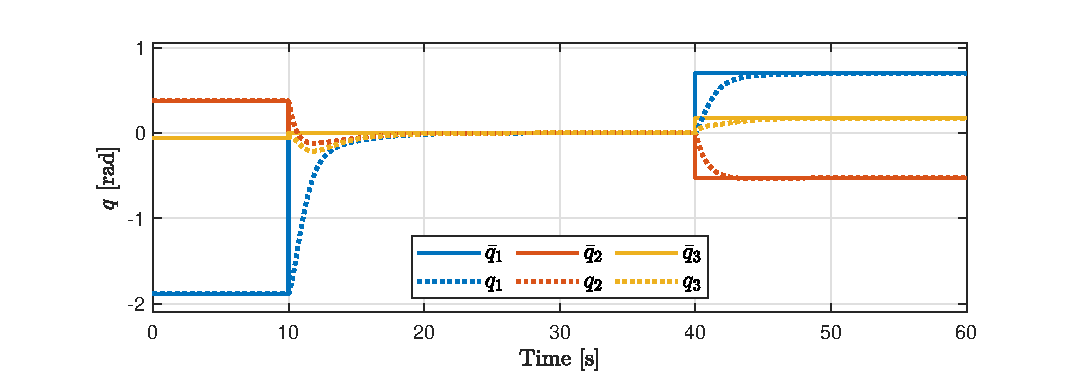
\includegraphics[width=0.33\textwidth, trim={0.75cm 0cm 0.75cm 0cm}]{backstepping/figures/time_series_plot_m_p-0.5_untuned_configuration_backstepping_v2.eps}}
  \subfloat[Piston position $\mu_\mathrm{p}$]{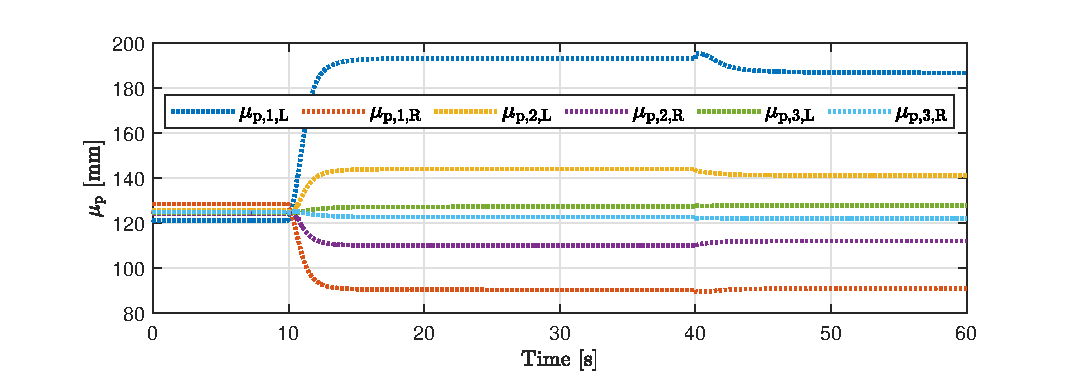
\includegraphics[width=0.33\textwidth, trim={0.75cm 0cm 0.75cm 0cm}]{backstepping/figures/time_series_plot_m_p-0.5_untuned_piston_position_backstepping_v2.eps}}
  \subfloat[Actuation force $f_\mathrm{p}$]{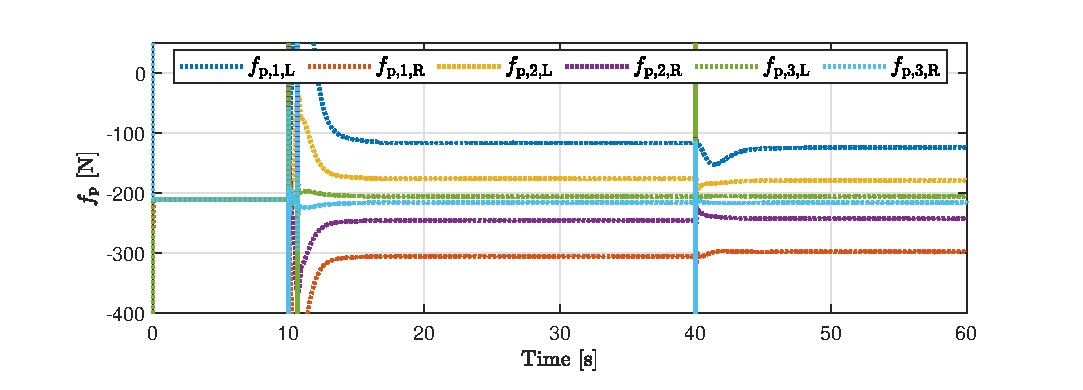
\includegraphics[width=0.33\textwidth, trim={0.75cm 0cm 0.75cm 0cm}]{backstepping/figures/time_series_plot_m_p-0.5_untuned_actuation_force_backstepping_v2.eps}}\\
  \caption{Simulation of posture regulation under \gls{PCC} approximation for an actuation system with increased inertia ($m_\mathrm{p} = \SI{0.5}{kg}$) comparing the performance of an end-to-end PID baseline controller (1st row), with a coupling-aware PID controller (2nd row) and the nonlinear backstepping controller (3rd row). The set-point reference configuration is shown with solid lines.}
  \label{fig:time_series_plots_m_p-0.5_untuned}
  \vspace{-0.5cm}
\end{figure*}
%
\begin{figure}[ht]
  \centering
  \subfloat[End-to-end PID]{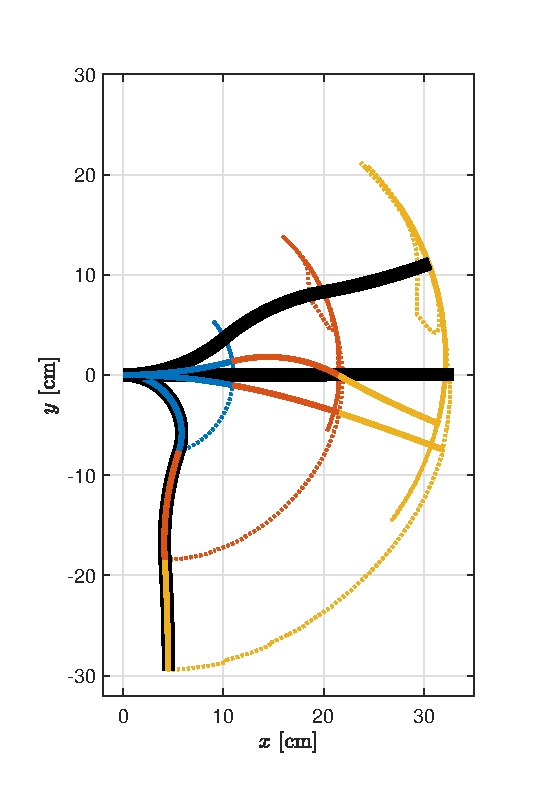
\includegraphics[width=0.33\columnwidth, trim={0.5cm 0 0.5cm 0}]{backstepping/figures/cartesian_evolution_plot_m_p-0.5_untuned_full_system_pid_v1.eps}\label{fig:cartesian_evolution_plot_m_p-0.5_untuned_full_system_pid}}
  \subfloat[Coupling-aware PID]{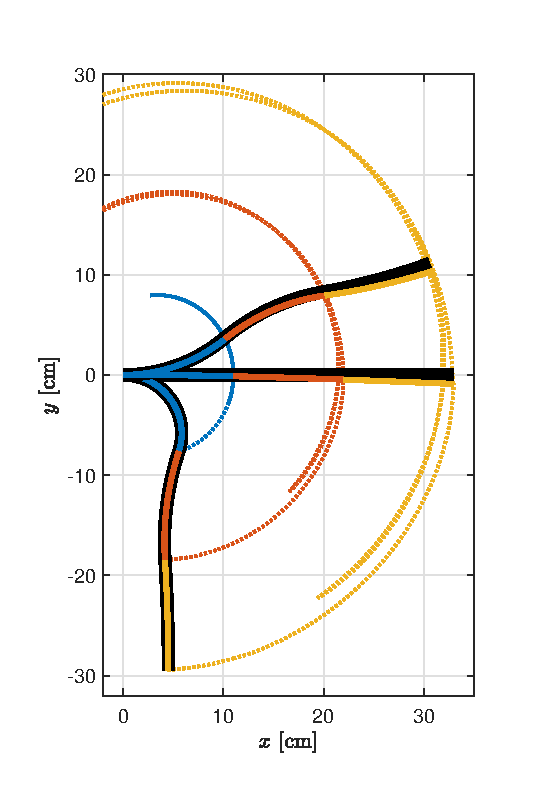
\includegraphics[width=0.33\columnwidth, trim={0.5cm 0 0.5cm 0}]{backstepping/figures/cartesian_evolution_plot_m_p-0.5_untuned_coupling_aware_pid_v1.eps}\label{fig:cartesian_evolution_plot_m_p-0.5_untuned_coupling_aware_pid}}
  \subfloat[Backstepping]{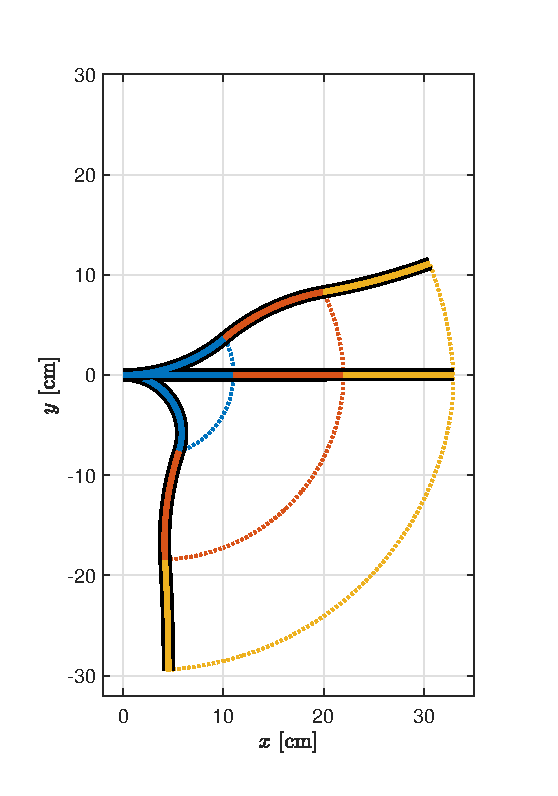
\includegraphics[width=0.33\columnwidth, trim={0.5cm 0 0.5cm 0}]{backstepping/figures/cartesian_evolution_plot_m_p-0.5_untuned_backstepping_v2.eps}\label{fig:cartesian_evolution_plot_m_p-0.5_untuned_backstepping}}
  \caption{Cartesian evolution of the soft robot for an actuation system with increased inertia ($m_\mathrm{p} = \SI{0.5}{kg}$). All gains remain unchanged and are tuned for the original system with $m_\mathrm{p} = \SI{0.19}{kg}$. The dotted lines mark the evolution of the tip of the segments. The soft robot consists of three segment (blue, orange and yellow). The reference configuration at the three set-points is marked with a thick black line.}
\end{figure}
%
\subsection{System}
%
We consider a planar soft robot arm consisting of three independently actuated CC segments, modeled upon the second half of the robot in \cite{della2020model}. % in Simulink. It is inspired by recent designs and models of similar pneumatically actuated continuum arms in literature~\cite{della2020model, marchese2014design}. 
%We model the 
Segments have equal length $l_{0} = \SI{11}{cm}$, uniform mass density $\rho = \SI{0.99}{kg \per m}$ concentrated on the central axis. % - resulting in \SI{109}{g} per segment. %We use the \gls{PCC} assumption~\cite{jones2006kinematics} to compute the Jacobian for any point along the center-line of the segment. The \gls{EoM} are derived using the Euler-Lagrange equation. We add an elastic term $K q$ with $K$ defined as a diagonal matrix with the elastic constant \SI{0.01}{N \per rad}. Natural damping is considered with $D \dot{q}$ and the diagonal damping constant \SI{0.01}{Ns \per rad}.
%
The stiffness $K$ and damping $D$ matrices are diagonal with constants \SI{0.01}{N \per rad} and \SI{0.01}{Ns \per rad}. The segment has a diameter of \SI{44.5}{mm}. Based on CAD analyses of a real system, we take $d_{\mathrm{C},\mathrm{a}} = \SI{7.14}{mm}$, $d_{\mathrm{C},\mathrm{b}} = \SI{20.19}{mm}$, and $b_\mathrm{C} = \SI{8.07}{mm}$.
%We set the parameters $d_{\mathrm{C},\mathrm{a}}$ and $d_{\mathrm{C},\mathrm{b}}$ as the inner and outer air chamber walls are placed at a radial distance of \SI{7.14}{mm} and \SI{20.19}{mm}. We analysed the chamber volume in CAD to be \SI{46.2}{cm^3}, which results in a modelled planar chamber depth of $b_\mathrm{C} = \SI{8.07}{mm}$.
%
%The base of the first segment is aligned with the x-axis and gravity is acting along the negative y-axis. 
A positive curvature and positive configuration $q_i$ correspond to bending counter-clockwise. 
% The base of the robot is oriented perpendicularly to gravity, so that it tends to induce clock-wise bending.
The straight configuration of the robot along the x-axis is perpendicular to gravity acting in negative y-direction as shown in Figure~\ref{fig:pcc_case_overview}, so that gravity tends to induce clock-wise bending.
%
%We were inspired by the fluidic drive cylinder designed by Marchese et al.~\cite{marchese2014design} in our choice of parameters for the pistons. Accordingly, 
Moving to the pistons, $A_\mathrm{p} = \SI{7.9}{cm^2}$, $m_\mathrm{p} = \SI{0.19}{kg}$, $l_\mathrm{p} = \SI{0.5}{m}$ are chosen.
% We model the cross-sectional area of the piston $A_\mathrm{p}$ as \SI{7.9}{cm^2}, the mass of the piston $m_\mathrm{p}$ with \SI{0.19}{kg} resulting in a diagonal mass matrix $M_\mathrm{p}$, the length of the piston $l_\mathrm{p}$ as \SI{0.5}{m} and 
We consider a damping matrix $D_\mathrm{p}$ with damping constants $d_\mathrm{p} = \SI{10}{\kilo \newton \second \per \meter}$ along the diagonal. The pistons are filled with air at $\mu_{\mathrm{p}, 0} = l_\mathrm{p}$ and $p_\mathrm{atm} = \SI{1}{bar}$ and subsequently pre-loaded to $\mu_{\mathrm{p}, \mathrm{t}0} = 0.25 \, l_\mathrm{p}$. % before the experiment is started.
We set the backstepping gains to $K_1 = \SI{6000}{\per \second}$ and $K_2 = \SI{4.5}{\kilo \newton \per \meter}$.

\subsection{End-to-end PID}
We first introduce an end-to-end PID controller, which will serve as a baseline
%
\begin{equation}\small
    \Delta f_\mathrm{p} = K_\mathrm{p} (\bar{q}-q) + K_\mathrm{i} \int_0^t (\bar{q}-q) \, \mathrm{d}t' - K_\mathrm{d} \, \dot{q}
\end{equation}
%
where $K_\mathrm{p},K_\mathrm{i},K_\mathrm{d} \geq 0$ are scalar gains. $\Delta f_\mathrm{p} \in \mathbb{R}^{n_q}$ is the scalar offset from the actuation force $f_{\mathrm{p},\mathrm{t}0}$ corresponding to the pre-loaded pressure $p_{\mathrm{t}0}$.
%
Analogue to \eqref{eq:dist_G_p_q_planar_pcc}, $\Delta f_\mathrm{p}$ can be equally distributed on both chambers within a segment.
% \begin{equation}\small
% \begin{split}
%     f_{\mathrm{p},\mathrm{L},i} = f_{\mathrm{p},\mathrm{t}0} + 0.5 \, \Delta f_{\mathrm{p},i}, \quad f_{\mathrm{p},\mathrm{R},i} = f_{\mathrm{p},\mathrm{t}0} - 0.5 \, \Delta f_{\mathrm{p},i}.
% \end{split}
% \end{equation}
The PID gains have been selected so to achieve a similar transient behaviour as for the backstepping controller % required lengthy heuristic tuning and the selection was guided by the Ziegler-Nichols method,
and are equal to $K_\mathrm{p} = \SI{200}{\newton \per \radian}$, $K_\mathrm{i} = \SI{7}{\newton \per \radian \per \second}$, and $K_\mathrm{d} = \SI{200}{\newton \second \per \radian}$. 
% Segment 1, 2 and 3 are weighted with gain multipliers of $1.5$, $1$, and $0.5$.

%
\subsection{Coupling-aware PID}
%
% We attempted implementing a standard low-level PID with static compensation as in \cite{della2020model} for fair comparison, but we could not find a set of gains that was stable when using \eqref{eq:high_level_regulation}.
Next, we implement a control strategy that takes advantage of the understanding of the potential coupling and uses a PID for low-level control of the pistons
%
\begin{equation}\small
    f_{\mathrm{p}} = K_\mathrm{p} \left (\Gamma(q, \bar{q})-\mu_\mathrm{p} \right ) +  K_\mathrm{i} \int_{0}^t \left ( \Gamma(q, \bar{q})-\mu_\mathrm{p} \right ) \mathrm{d}t' - K_\mathrm{d} \, \dot{\mu}_\mathrm{p}.
\end{equation}
%
Here, $K_\mathrm{p},K_\mathrm{i},K_\mathrm{d} \geq 0$ are scalar gains, and $\Gamma(q, \bar{q})$ is the correction on \eqref{eq:high_level_regulation} which takes the coupling defined in \eqref{eq:gamma} in account. 
%
The PID gains are tuned similarly to the coupling-aware PID
and are equal to $K_\mathrm{p} = \SI{150 000}{\newton \per \meter}$, $K_\mathrm{i} = \SI{15 000}{\newton \per \meter \per \second}$, and $K_\mathrm{d} = \SI{100}{\newton \second \per \meter}$. 
% Segment 1, 2 and 3 are weighted with gain multipliers of $1.5$, $1$, and $0.5$.  %~\cite{ziegler1942optimum}.

\subsection{Results}

We simulate the response of the closed loop generated by all three controllers to a sequence of step references. The segments are initialised at the equilibrium configuration. % of the system $\begin{bmatrix} \SI{-1.8850}{\radian} & \SI{0.3752}{\radian} & \SI{-0.0593}{\radian} \end{bmatrix}^\mathrm{T}$, where they are for \SI{10}{s}. 
At \SI{10}{s}, the reference is moved to the straight configuration $\bar{q} =  0$. After another \SI{30}{s}, we change it again to $\bar{q} = \begin{bmatrix} \SI{0.6981}{\radian} & \SI{-0.5236}{\radian} & \SI{0.1745}{\radian} \end{bmatrix}^\mathrm{T}$.
% We choose an \emph{ode45} with variable step size and a max step size of $0.001$ for our Simulink simulation. %To avoid numerical instabilities of the PCC formulation close to a straight configuration, we use $\tilde{q}$  with $\lvert \tilde{q}_i \rvert = \max (q_i, \SI{3}{\degree})$ as the input into the \gls{EoM} and the controller formulations.

Figure~\ref{fig:time_series_plots} shows that the backstepping controller is approaching the set-point reference with no oscillations nor overshooting. These are instead visible for coupling-are PID controller after the second change in reference configuration. 
The end-to-end PID controller does not converge to the desired configuration within \SI{60}{s} as it does not take into account gravity.

Next, we increase the inertia of the actuation system by setting the piston mass $m_\mathrm{p}$ to \SI{0.5}{kg}. We leave both the backstepping and the PID gains unchanged. Figures~\ref{fig:time_series_plots_m_p-0.5_untuned}-\ref{fig:cartesian_evolution_plot_m_p-0.5_untuned_full_system_pid} demonstrate that the backstepping-based approach is able to adapt to the new system, while the end-to-end PID shows large oscillations at \SI{50}{s} and the coupling-aware PID displays significantly overshoot in curvatures and piston positions. 
Note that the latter are especially dangerous in real experiments, since they may signify that pistons reaches their limits.

% \begin{table*}
% \centering
% \caption{System parameters used in simulations}
% \vspace{0.25cm}
% \begin{tabular}{c c c c c c c c c c}\toprule
% $l$ & $\rho$ & $k$ & $d$ & $b_\mathrm{C}$ & $d_{\mathrm{C},a}$ & $d_{\mathrm{C},b}$ & $A_\mathrm{p}$ & $l_\mathrm{p}$ & $m_\mathrm{p}$\\
% \midrule
% \SI{110}{mm} & \SI{0.99}{g \per mm} & \SI{0.01}{N \per \radian} & \SI{0.01}{Ns \per \radian} & \SI{8.07}{mm} & \SI{7.14}{mm} & \SI{20.19}{mm} & \SI{7.9}{cm^2}~\cite{marchese2014design} & \SI{0.5}{m} & \SI{0.19}{kg}~\cite{marchese2014design}\\
% \bottomrule
% \end{tabular}
% \label{tab:system_parameters}
% \end{table*}